\begin{frame}

\frametitle{\D{}, values and shapes}

\begin{columns}

\column{0.3\textwidth}
\begin{center}
$$b\in\mathbb{B}$$
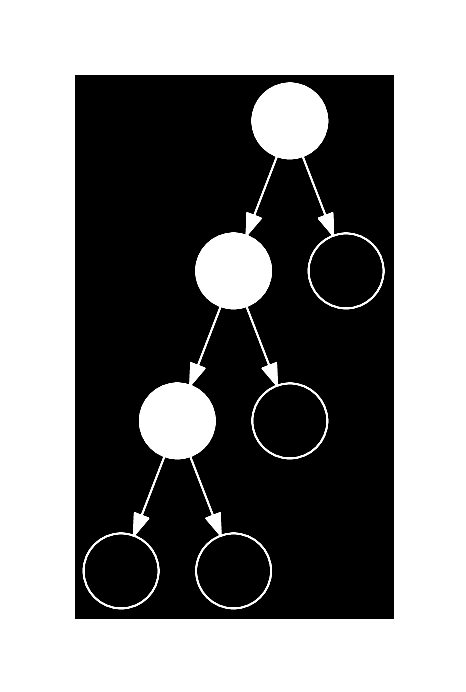
\includegraphics[scale=0.5]{figures/value}
\end{center}

\column{0.3\textwidth}

\begin{center}
{\fontsize{40}{20}$\succ$}
\end{center}

\column{0.3\textwidth}

\begin{center}
$$s\in\mathbb{S}$$
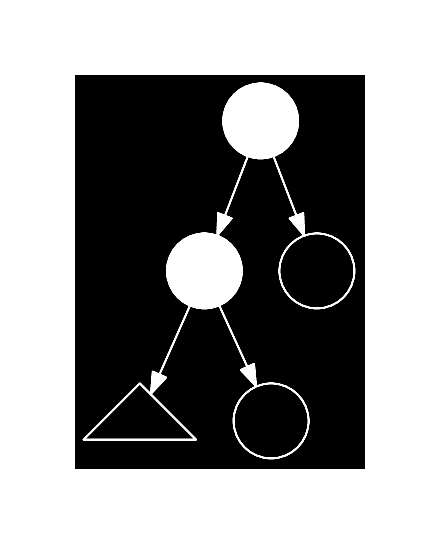
\includegraphics[scale=0.5]{figures/shape}
\end{center}

\end{columns}

\end{frame}

\begin{frame}

\frametitle{\D{}, shapes and shapes}

\begin{columns}

\column{0.3\textwidth}
\begin{center}
$$s_1\in\mathbb{S}$$
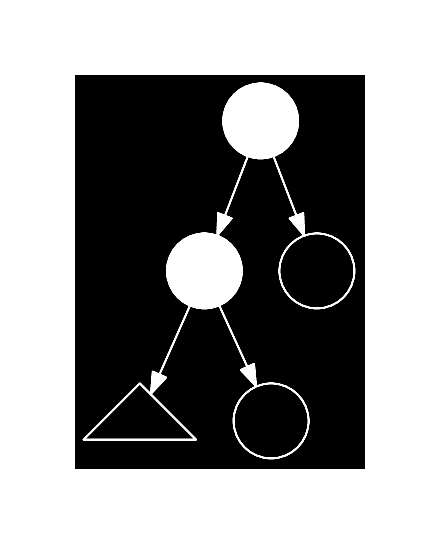
\includegraphics[scale=0.5]{figures/shape}
\end{center}

\column{0.3\textwidth}

\begin{center}
{\fontsize{40}{20}$\succ$}
\end{center}

\column{0.3\textwidth}

\begin{center}
$$s_2\in\mathbb{S}$$
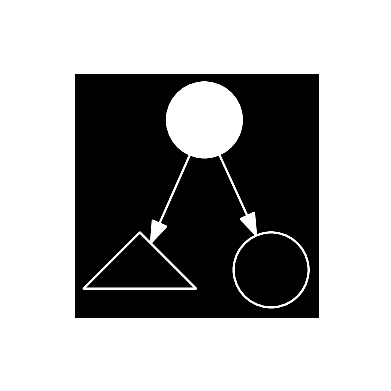
\includegraphics[scale=0.5]{figures/shape-2}
\end{center}

\end{columns}

\end{frame}

\begin{frame}

\frametitle{Disjoint shapes}

\begin{center}

$$s_1\cap s_2=\emptyset\quad\text{iff}\quad B_1\cap B_2=\emptyset$$

where

$$s_1,s_2\in\mathbb{S} \wedge B_1=\{b\mid b\in\mathbb{B} \wedge b\succ
s_1\}\wedge B_2=\{b\mid b\in\mathbb{B} \wedge b\succ s_2\}$$

\end{center}

\end{frame}

% TODO: All patterns now have a name.

\begin{frame}[fragile]

\begin{lstlisting}
data Pattern
  = PNil
  | PVariable String
  | PNode Pattern Pattern

getSiblings :: Pattern -> [Pattern]

getSiblings PNil =
  [PNode (PVariable "_") (PVariable "_")]

getSiblings (PVariable _) = []

getSiblings (PNode leftP rightP) =
  let
    leftS = getSiblings leftP
    rightS = getSiblings rightP
    leftInit = map (\s -> PNode leftP s) rightS
    rightInit = map (\s -> PNode s rightP) leftS
  in
    [PNil] ++
      leftInit ++ rightInit ++
      interleaveSiblings name leftS rightS
\end{lstlisting}

\end{frame}
